\section{Middleware}
\subsection{Indexstruktur}

\subsubsection{Anforderungen}
Der Index soll eine effiziente Suche nach Mutationen für das Frontend ermöglichen. Während des Programmstarts wird der Index aus der vorhandenen Datenbank aufgebaut und steht dann so lange zur Verfügung, bis das Programm beendet wird.
Im Index wird mit Intervallgrenzen gesucht und der Index gibt alle Intervalle zurück, die komplett innerhalb des angegebenen Intervalls liegen.\\
Der Index wird verteilt aufgebaut und liegt auf 4 virtuellen Maschinen verteilt. Die für den Index spezifizierten Funktionen sprechen immer einen Teilindex an. Der Aufruf der Funktionen wird über den IndexController erfolgen, der immer alle 4 Teilindizes ansprechen wird.
\subsubsection{Funktionen und Datenstrukturen}
Die Funktionen des Indexes variieren in ihrerem Ablauf je nach gewählter Indexstruktur. Momentan existieren 3 Varianten, die getestet werden. Es ist nicht ausgeschlossen, dass weitere Strukturen im Laufe der Entwicklung getestet werden. Da die Dauer des Indexaufbaus für den Endnutzer nicht relevant ist hängt die Auswahl der letztendlich genutzten Struktur lediglich von der Geschwindigkeit der Suchanfragen ab.
Im folgenden werden die Such-und Einfüge-Operationen basierend auf den jeweiligen Indexstrukturen beschrieben
\newpage
\hfill\\
\textbf{IntervallTree}\\
In diesem Fall basiert die Indexstruktur auf einem Intervallbaum.\\
Hierfür wird die frei zugängliche Bibliothek "IntervallST.java" der Universität Princeton genutzt. Beide Funktionen haben hier lediglich die Aufgabe als Interface zu den zugehörigen Bibliotheksfunktionen zu dienen: contains() zur Suche und put() zum Einfügen.\\
Das Suchergebnis wird nach möglichen Filtern gefiltert. Bei n Intervallen und einer Such-Ergebnisliste der Größe m ergibt sich ein Komplexität von O(log n + m)\\ Die Bibliothek muss noch angepasst werden, damit das Einfügen von gleichen Intervallen möglich ist ohne, dass das zuerst eingefügte Intervall gelöscht wird.
\begin{algorithm}
search()\\{
found intervalls = contains(intervall)\;
\ForAll{elements in found intervalls}
{
{\If{element corresponds to specified filters}
{add element to answer list\;}
}
return answer list\;
}
}
\end{algorithm}


\begin{algorithm}
addMutation()\\{
\If{mutation is already in index}
{return "index already contains mutation"\;}
put()\;
return \enquote{added mutation}\;
}
\end{algorithm}

\newpage
\hfill\\
\textbf{Suchbaumbasierter Index}\\
Da ein Großteil der Intervalle einstellig bzw sehr kurz sind bietet sich ein einfacher binärer Suchbaum als Datenstruktur an.\\
Dieser wird um einen Iterator erweitert, damit effizient eine Menge an Knoten ausgewählt werden kann.\\
Hierfür wird die Java-Klasse TreeMap verwendet, die eine Suche in logarithmischer Zeit ermöglicht. Die Ergebnismenge wird einmal durchlaufen, Mutationen deren Endpunkt außerhalb des gesuchten Intervalls liegen werden dabei entfernt und jeder Knoten wird nach den angegebenen Filtern gefiltert. Bei n Intervallen und einer Such-Ergebnismenge von m Intervallen ergibt sich eine Laufzeit von O(log n +m).\\
Auch in dieser Implementation dienen die Funktionen als Interface zu den jeweiligen Funktionen der genutzten Klasse: submap() zur Suche und put() zum Einfügen von Objekten).
\begin{algorithm}
search()\\{
found intervalls = submap(intervall)\;
\ForAll{elements in found intervalls}
{
{\If{element corresponds to specified filters}
{add element to answer list\;}
}
return answer list\;
}
}
\end{algorithm}


\begin{algorithm}
addMutation()\\{
\If{mutation is already in index}
{return \enquote{index already contains mutation}\;}
put()\;
return \enquote{added mutation}"\;
}
\end{algorithm}

\newpage\hfill\\
\textbf{Arraybasierter Index}\\
Sollte die Anzahl der Mutationen groß genug sein, dass sie mit Integer-Variablen darstellbar ist, so bietet sich unter Umständen auch ein arraybasierter Index an.\\
Dieser speichert alle Mutationen aufsteigend sortiert nach ihrem Anfangspunkt.
Wird nun nach einem Intervall gesucht, so iteriert er über das Array beginnend bei der Mutation, deren Startwert noch im gesuchten Intervall liegt. Dabei wird für jede Mutation überprüft, ob ihr Endwert noch im gesuchten Intervall liegt. Ist dem so wird sie zur Ergenismenge hinzugefügt. Hierbei können auch direkt die Filter überprüft werden.\\
Es so lange iteriert, bis der Startwert aller folgenden Mutationen größer, als der vom Nutzer angegebene Endwert ist.\\
Falls Mutationen an der gleichen Stelle beginnen, so verschieben sich alle folgenden Mutationen in der Liste, da in aufeinanderfolgenden Zellen gleiche Startintervalle gespeichert werden müssen. Es muss also ermittelt werden, wo sich die erste im Intervall liegende Mutation befindet. Ein Verfahren hierfür wird noch ermittelt\\
Bei m Mutationen, deren Startwert sich im gesuchten Intervall befinden, liegt die Laufzeit bei O(m + $\epsilon$), wobei $\epsilon$ davon abhängt, wie die erste Mutation ermittelt wird. Es kann aber davon ausgegangen werden, dass $\epsilon$ einen geringen Anteil an der Laufzeit ausmachen wird.
\begin{algorithm}
search()\\{
find index x of first mutation that lies in intervall\;
\While{starting point of mutation at index x lies in search intervall}
{{\If{endpoint of mutation at index x lies in search intervall and mutation corresponds to specified filters}
{add mutation to answer list\;}
}
x=x+1\;
}
return answer list\;}

\end{algorithm}


\begin{algorithm}
addMutation()\\{
\If{mutation is already in index}
{return "index already contains mutation"\;}
insert mutation at corresponding index and adjust array properly\;
return \enquote{added mutation}\;}
\end{algorithm}
\newpage
\subsection{IndexController}
\subsubsection{Anforderungen}
Der IndexController nimmt Suchanfragen entgegen, leitet diese an die 4 Teilindizes weiter und fügt die Teilergebnisse wieder zusammen.\\Falls eine Anfrage intern in mehrere Teilanfragen aufgeteilt werden sollte, weil z.B. ein Gen, nach dem gesucht wird an mehreren Stellen auftreten kann, leutet der IndexController alle Teilanfragen sequentiell an die Indizes weiter, fügt die Teilergebnisse zusammen und schickt die Ergebnismenge an den QueryReceiver zurück.
\subsubsection{Funktionen}
\textbf{answerQuery(int[] intervals,String[] Sources,int[]filter)}
Die Funktion erhält mehrere Listen als Parameter, die die nötigen Informationen für die einzelnen Anfragen beinhalten. Jeweils 2 aufeinanderfolgende Einträge in der Intervall-Liste beschreiben den Start-und Endpunkt der gesuchten Intervalle. Die Einträge in den anderen Listen werden für alle Anfragen genutzt\\
Die Anfragen werden sequentiell an die 4 Teilindizes weitergeleitet und einzelnen Ergebnisse konkateniert und in einer Liste zurückgegeben.
\begin{algorithm}
\ForAll{queries in parameter list}
{\ForAll{sub indices}
{answer list = index.search()\;}
concatenate all answer lists\;
}
concatenate answer lists of each sub query\;
return answer list\;
\end{algorithm}
\\
\textbf{buildIndex()}
Die Funktion wird bei Programmstart ausgeführt und baut auf Basis der Datenbank die 4 Teilinidzes auf.\\
Für jede Mutation wird zufällig entschieden in welchen Index sie eingefügt wird.\\
\begin{algorithm}
\ForAll{elements in database}
{\If{element is already in index}
{skip element\;}
choose which sub index to insert into\;
index.addMutation()\;
}
return "index built"\;
\end{algorithm}

\newpage
\subsection{Klassen-Diagramm}
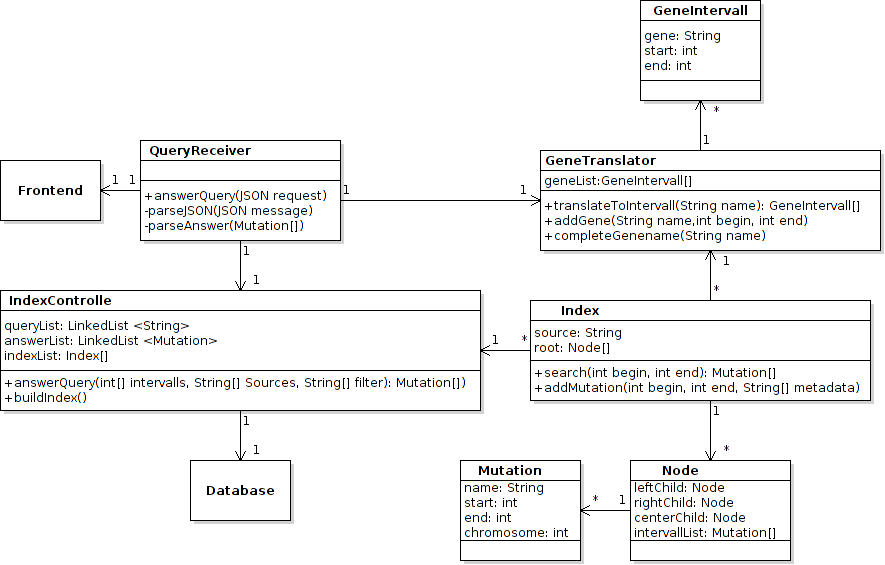
\includegraphics[width=\textwidth]{middleware/Middleware_class_3rd_Revision.png}

\newpage
\subsection{Sequenzdiagramme}
\subsubsection{Intervall-Suche}
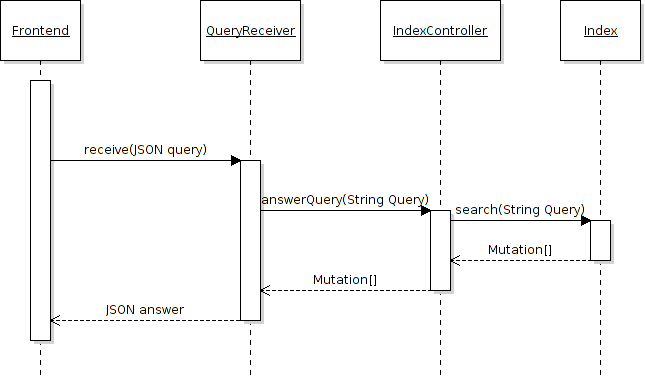
\includegraphics[width=\textwidth]{middleware/intervall_seq.png}
\subsubsection{Names-Suche}
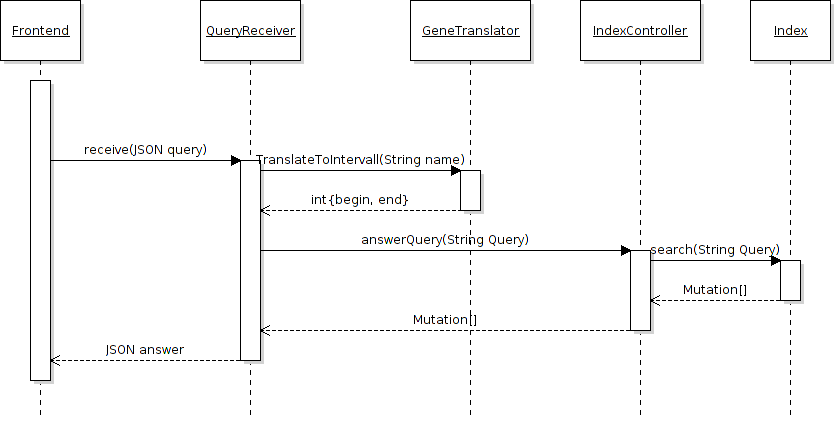
\includegraphics[width=\textwidth]{middleware/namesearch_seq.png}
\subsubsection{Suche nach Gennamen}
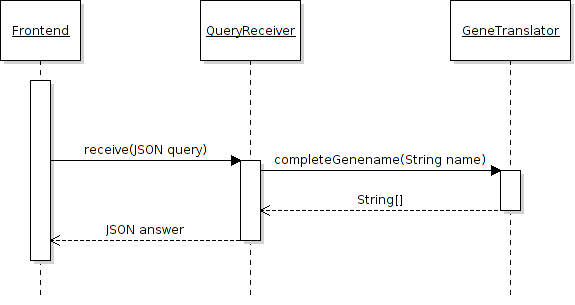
\includegraphics[width=\textwidth]{middleware/prefix_seq.png}

\newpage
\subsection{Unit-Tests}
\subsubsection{QueryReceiver}
\textbf{Testfall 1 - erfolgreiche Intervallanfrage ohne Metadaten}
\begin{verbatim}
  Eingabe
{
  "source": The Cancer Atlas,\usepackage[utf8]{inputenc}
  "chromosome": 3,
  "position": {"from": 100, "to": 200},
  "zoom": 1,
  "subindex": ,
  "hasDetail": (false)
}

  Ausgabe
{
  {
    "source:" The Cancer Atlas,
    "chromosome": 3,
    "position": {"from": 100, "to": 200},
    "details": { "refseq": ,
                "mutations": [{ "name": ,
                                "position": {"from": , "to": },
                                "metadata":
                              },]},
    "graph": {
              { "subintervall": Anzahl der Subintervalle,
                "counts": Anzahl der Ergebnisse
              }
            }
  }
}
\end{verbatim}
\textbf{Testfall 2 - erfolgreiche Intervallanfrage mit Metadaten}
\begin{verbatim}
  Eingabe
{
  "source": The Cancer Atlas,
  "chromosome": 3,
  "position": {"from": 100, "to": 200},
  "zoom": 1,
  "subindex": ,
  "hasDetail": (true)
}

  Ausgabe
{
  {
    "source:" The Cancer Atlas,
    "chromosome": 3,
    "position": {"from": 100, "to": 200},
    "details": { "refseq": Referenzsequenz,
                "mutations": [{Mutation1},{Mutation2},...]},
    "graph": {
              { "subintervall": ,
                "counts":
              }
            }
  }
}
\end{verbatim}
\textbf{Testfall 3 - erfolglose Intervallanfrage}
\begin{verbatim}
  Eingabe
{
  "source": The Cancer Atlas,
  "chromosome": 3,
  "position": {"from": 100, "to": 200},
  "zoom": 1,
  "subindex": ,
  "hasDetail": (true)
}

  Ausgabe
{
  {
    "source:" The Cancer Atlas,
    "chromosome": 3,
    "position": {"from": 100, "to": 200},
    "details": { "refseq": ,
                "mutations": ...},
    "graph": {
              { "subintervall": ,
                "counts":
              }
            }
  }
}
\end{verbatim}
\newpage\hfill\\
\textbf{Testfall 4 - erfolgreiche Namensanfrage}
\begin{verbatim}
  Eingabe
{
  "source": The Cancer Atlas,
  "chromosome": 3,
  "search": "Gen im Cancer Atlas"
}

  Ausgabe
{
  "source": The Cancer Atlas,
  "chromosome": 3,
  "search": "Gen im Cancer Atlas",
  "position": {"from": Startposition, "to": Endposition}
}
\end{verbatim}
\textbf{Testfall 5 - erfolglose Namensanfrage}
\begin{verbatim}
  Eingabe
{
  "source": The Cancer Atlas,
  "chromosome": 3,
  "search": "Gen, dass nicht im Cancer Atlas ist"
}

  Ausgabe
{
  "source": The Cancer Atlas,
  "chromosome": 3,
  "search": "Gen im Cancer Atlas",
  "position": " "
}
\end{verbatim}
\textbf{Testfall 6 - fehlerhafte Anfrage}
\begin{verbatim}
  Eingabe
{
  "source": ""
}

  Ausgabe
{
  "answer": "unknown format"
}
\end{verbatim}
\newpage
\subsubsection{GeneTranslator}
Der GeneTranslator hat 2 Aufgaben. Zum einen soll er während der Indexerstellung mit Inhalt (also Gennamen und zugeörigen Intervallen) befüllt werden, zum anderen soll eine Suche nach Gennamen in ihm möglich sein.\\
\\
\textbf{Testfall 1 - addGene - Einfügen in Datenstruktur}\\
Eingabe: Testgen, 350, 500\\
Ausgabe: Dass Gen sollte in den Baum eingefügt sein und per searchForGene() findbar sein\\
\\
\textbf{Testfall 2 - addGene - Doppeltes Einfügen in Datenstruktur}\\
Eingabe: Testgen, 350, 500\\
		 Testgen, 350, 500\\
Ausgabe: Dass Gen sollte nur einmal in die Datenstruktur eingefügt werden. Ausgabe, dass das Gen bereits in der Struktur vorhanden ist.\\
\\
\textbf{Testfall 3 - addGene - Aufruf ohne Parameter}\\
Eingabe: [...]\\
Ausgabe: Fehlermeldung über  parameterlosen Aufruf\\
\\
\textbf{Testfall 4 - tranlateToIntervall - erfolgreiche Suche}\\
Eingabe: Testgen (befindet sich bereits in Datenstruktur)\\
Ausgabe: 350, 500\\
\\
\textbf{Testfall 5 - tranlateToIntervall - erfolglose Suche}\\
Eingabe: Testgen2 (befindet sich nich in Datenstruktur)\\
Ausgabe: Fehlermeldung über erfolglose Suche\\
\\
\textbf{Testfall 6 - tranlateToIntervall - Aufruf ohne Parameter}\\
Eingabe: [...]\\
Ausgabe: Fehlermeldung über Parameterlosen Aufruf\\
\\
\textbf{Testfall 7 - completeGeneName - erfolgreiche Suche mit einem Ergebnis}\\
Eingabe: Test (Testgen1 befindet sich bereits in Datenstruktur)\\
Ausgabe: Testgen1\\
\\
\textbf{Testfall 8 - completeGeneName - erfolgreiche Suche mit mehreren Ergebnissen}\\
Eingabe: Test (Testgen1 und Testgen2 befinden sich bereits in Datenstruktur)\\
Ausgabe: Testgen1, Testgen2\\
\\
\newpage\hfill\\
\textbf{Testfall 9 - completeGeneName - erfolglose Suche}\\
Eingabe: Test (Es befindet sich kein Gen mit Präfix Test in der Datenstruktur)\\
Ausgabe: Fehlermeldung über erfolglose Suche
\subsubsection{IndexController}
\textbf{Testfall 1 - answerQuery - einfache Intervallanfrage}\\
Eingabe: 1,3,100,200\\
Ausgabe: zum Intervall gehörende Mutationsobjekte\\
\\
\textbf{Testfall 2 - answerQuery - komplexere Intervallanfrage}\\
Eingabe: 1,3,100,200 ; 1,3,150,350\\
Ausgabe: eine Mutationsliste mit den Ergebnissen beider Anfragen\\
\\
\textbf{Testfall 3 - answerQuery - unvollständige Intervallanfrage}\\
Eingabe: 1,100,200\\
Ausgabe: Fehlermeldung über unvollständige Anfrage\\
\\
\textbf{Testfall 4 - answerQuery - leere Anfrage}\\
Eingabe: [...]\\
Ausgabe: Fehlermeldung über leere Anfrage\\
\\
\textbf{Testfall 5 - answerQuery - überspezifizierte Intervallanfrage}\\
Eingabe: 1,3,100,200,300,400\\
Ausgabe: Fehlermeldung über überspezifizierte Anfrage\\
\\
\textbf{Testfall 6 - buildIndex - erfolgreicher Indexaufbau}\\
Eingabe: [...] (Datenbank ist erreichbar)\\
Ausgabe: Erfolgreich gebauter Index\\
\\
\textbf{Testfall 7 - buildIndex - erfolgloser Indexaufbau}\\
Eingabe: [...] (Datenbank ist nicht erreichbar)\\
Ausgabe: Fehlermeldung über erfolglosen Indexaufbau
\newpage
\subsubsection{Intervallbaum}
\textbf{1. Intervalle einfügen:}\\
Das Intervall muss im Baum an der richtigen Stelle eingefügt werden und der Baum muss gegebenenfalls neu balanciert werden (z.B. wie ein AVL-Baum).\\\\
Bsp.: Einfügen des Intervalls [12,15]\\\\
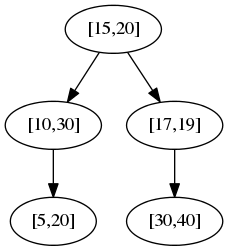
\includegraphics[width=0.2\textwidth]{middleware/Testfaelle/1.png}$~~~~~~~~~~~$
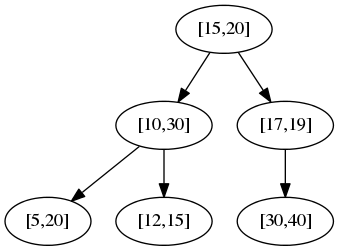
\includegraphics[width=0.3\textwidth]{middleware/Testfaelle/2.png}\\\\
\textbf{2. Intervall mit Startpunkt $>$ Endpunkt einfügen:}\\
Wenn ein Intervall (S,E) mit S$>$E eingefügt wird, dann sollte unser Programm eine Fehlermeldung ausgeben und darauf hinweisen, dass die Grenzen für das Intervall nicht korrekt sind.\\\\
Bsp.: Einfügen des Intervalls [20,10] in einen beliebigen Baum.\\\\
\textbf{3. Intervall mit Start- bzw. Endpunkt außerhalb des betrachteten Zahlenbereichs:}\\
Wenn ein Intervall in dem Baum eingefügt werden soll, das teilweise oder vollständig außerhalb unseres Zahlenbereichs liegt (Länge des Genoms), dann muss es eine Fehlermeldung geben, die dem Nutzer mitteilt, dass der gültige Zahlenbereich überschritten wurde.\\\\
Bsp.: Einfügen des Intervalls [-5,7] in einen beliebigen Baum.\newpage\hfill\\
\textbf{4. Schon vorhandenes Intervall einfügen:}\\
Duplikate sollen von unserem Baum nicht gespeichert werden, d.h. es wird kein neuer Knoten hinzugefügt, sondern die Informationen (bei uns also Pointer auf Dateien) des neuen Knotens müssen im bereits vorhandenen Knoten mitgespeichert werden.\\\\
Bsp.: Einfügen des Intervalls [15,20] in den folgenden Baum\\\\
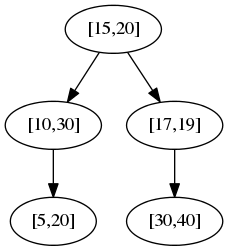
\includegraphics[width=0.2\textwidth]{middleware/Testfaelle/1.png}\\
\textbf{5. Suche nach vorhandenem Intervall:}\\
Bei der Suche sollen alle Intervalle ausgegeben werden, die das gesuchte Intervall in irgendeinem Punkt überlappen.\\\\
Bsp.: Suche im folgenden Baum\\\\
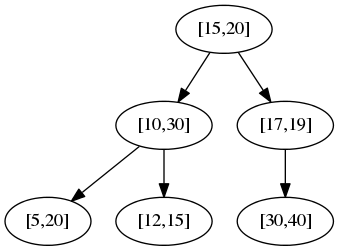
\includegraphics[width=0.3\textwidth]{middleware/Testfaelle/2.png}\\\\Suche [4,5] $\Rightarrow$ gib [5,20] aus\\
Suche [25,35] $\Rightarrow$ gib [10,30] und [30,40] aus\\
Suche [20,20] $\Rightarrow$ gib [15,20] und [5,20] aus
\subsection{Stresstests}
Der Stresstest hat zum Ziel herauszufinden, wie lange die durchschnittliche Query-Laufzeit ist.\\
Ziel des Systems ist es eine Laufzeit von unter einer Sekunde zu erreichen.\\
Um dies zu überprüfen werden mehrere Anfragen der gleichen Art (Intervallsuche, Gennamenssuche, Präfixsuche) sequentiell gestellt und die Antwortzeit gemessen. Alle Anfragen sollen in unter einer Sekunde eine Antwort erzielen.

